\subsection{Latency Encoding}

\textbf{Latency Encoding:}

\begin{wrapfigure}{r}{0.25\textwidth}
    \centering
    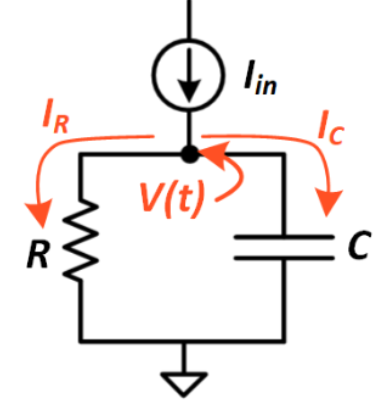
\includegraphics[width=0.25\textwidth]{methods/spike-encoding/graphs/LIF-circuit.png}
    \caption{RC circuit}
    \label{image:LIF_circuit}
  \end{wrapfigure}

Let's have another look at the RC circuit model used to modulate the behavior of a LIF neuron. This model gives us an equation we have seen before:

\begin{equation}
    I_{\text{in}} = I_R + I_C
\end{equation}

\begin{equation}
    I_{\text{in}} = \frac{1}{R} \cdot V_{\text{out}} + C \cdot \dot{V}_{\text{out}}
\end{equation}

\begin{equation}
    \tau = R \cdot C
\end{equation}


The result we computed earlier for constant input (for $v_{\text{th}} = 1, R = 1$) is:

\begin{wrapfigure}{r}{0.35\textwidth}
    \centering
    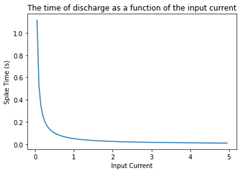
\includegraphics[width=0.35\textwidth]{methods/spike-encoding/graphs/exponential-decay.png}
    \caption{RC circuit}
    \label{image:exponential_decay}
\end{wrapfigure}

\begin{equation}
    v(t) = I_{\text{in}} \cdot \left(1 - \exp\left(-\frac{t}{\tau}\right)\right)
\end{equation}

A spike occurs when $v(t) = v_{\text{threshold}} \implies t_{\text{spike}}(I_{\text{in}}) = -\tau \cdot \ln\left(\frac{I_{\text{in}}}{I_{\text{in}} - v_{\text{threshold}}}\right)$.

We can use that equation to encode $X \in \mathbb{R}_{\geq 0}^{M \times N}$ data into $T \in \mathbb{R}_{\geq 0}^{M \times N}$ latency vector, which represents the spike time of each input neuron. In other words, each input neuron represents a different pixel in the image.

Another thing we need to take into consideration is the normalization of the image's values before the encoding. We can do it by setting a normalization factor $I_0$ such that 
\begin{equation}
V_{\text{normalized}} = \frac{I_0}{\max(V)} \cdot V
\end{equation}

The trial's max time $T$ will serve as a threshold for small values because inputs whose values will inspire a spike after the trial ends will be ignored, i.e. $I_{\text{th}} = \frac{v_{\text{th}}}{1 - \exp\left(-\frac{T}{\tau}\right)} \implies \forall I > I_{\text{th}}, t_{\text{spike}}(I) > T$.

The minimum time $\Delta T$ which we allow a spike is:
\begin{equation}
I_0 = \frac{v_{\text{th}}}{1 - \exp\left(-\frac{\Delta T}{\tau}\right)}
\end{equation}

But a problem is at hand: the distribution of the values of each image is problematic.

\begin{figure}[H]
    \centering
    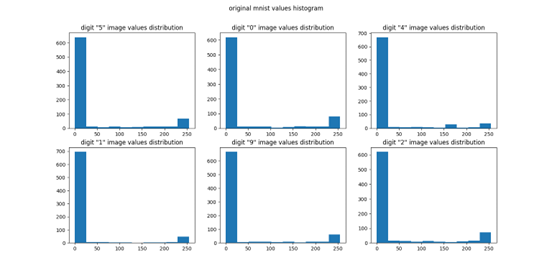
\includegraphics[width=0.8\textwidth]{methods/spike-encoding/graphs/mnist-values-histogram.png}
    \caption{histograms of the pixel values of random Mnist images divided into 10 bins}
    \label{fig:mnist-values-histogram}
\end{figure}

The fact that most values are 0's is not an issue; quite the opposite, we aim for sparsity. But the problem is that most values are distributed over 2-3 significant values. Another problem is that a linear normalization with logarithmic encoding is unable to distinguish close by values.

The resulting raster plot of the encoding expresses this issue:

\begin{figure}[h]
    \centering
    % Insert raster plot figure here
\end{figure}

To fix it, we suggest linear latency encoding by:
\begin{equation}
t(I_{\text{in}}) = -\tau \cdot \left(R \cdot I_{\text{in}} - V_{\text{thr}}\right)
\end{equation}

And clipping the zero values (they hold no useful information). The green lines represent the $\tau$ value, and the red lines represent $v_{\text{thr}}$.

And as we can see, the results are significantly improved.
